\section{Metod} 

Nedan följer en beskrivning av de arbetsmetoder vi använt oss utav och de mjukvaror och kodbibliotek som vi använt oss utav i projektet. 

\subsection{Arbetsmetodik}

% modulbaserat arbete..
Det upptäcktes tidigt att arbetet kunde delas upp i tre separata moduler; parser, interpretator och typcheckare. Dessa tre moduler intergrerar enbart med varandra genom det abstrakta syntaxträdet. Detta medför att det är väldigt lätt att utveckla de olika modulerna helt frånskilt från varandra. Figur \ref{fig:parser_steg} visar hur denna interaktion mellan de olika modulerna är tänkt att gå till. Figur \ref{fig:parser_steg} visar även att webbläsaren kommunicerar genom ett Javascript API och det abstrakta syntaxträdet och inte direkt med de olika komponenterna. 

\begin{figure}[h]
    \begin{center}
        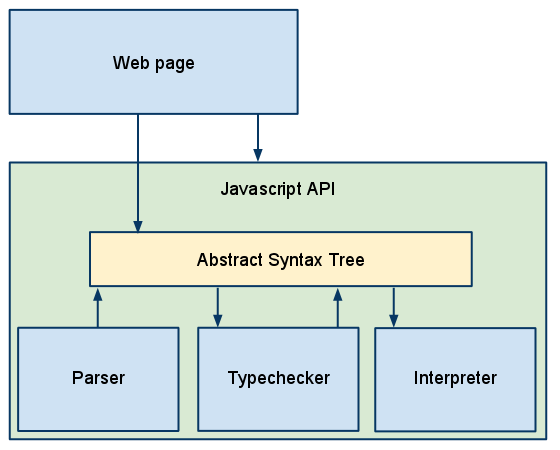
\includegraphics[width=1.0\textwidth]{image1.png}
        \caption{Överblick över tolkens struktur och interaktion}
        \label{fig:tolkens_struktur} % Labels must come after caption!
    \end{center}
\end{figure}


Arbetssättet präglades utav en iterativ utvecklingsmetodik med korta utvecklingscyklar. Arbetet delades upp med huvudansvarstagande över var sin modul och utfördes parallellt med varandra. Arbetet skedde dock framförallt i samlad grupp på grund av att det var många designrelaterade problem vi var tvugna att ta ställning till under projektet, till exempel hur vårat abstrakta syntaxträd skulle se ut, och för att det skulle bli enklare när vi skulle börja sammanfoga våra olika moduler med varandra. 
Det var också ett bra sätt att snabbt få hjälp av varandra eftersom vi ej exakt hur modulerna skulle se ut när vi påbörjade arbetet. Vi fann det därför praktiskt att använda en iterativ modell för att bit för bit utvigda våra moduler. 

Eftersom vi arbetade parallellt med olika moduler var vi beroende av ett bra versionshanteringssystem. Bra i vårt fall innebar att det skulle vara enkelt att arbeta i olika grenar, en gren för varje modul, och att det skulle gå snabbt och enkelt att slå ihop dessa förgreningar när vi behövde länka samman två utvecklares arbeten. I början av projektet använda vi oss utav SVN (Subversion). Detta berodde framförallt på att det var det versionshanteringssystem som alla i gruppen hade erfarenhet från tidigare. Dock insåg vi att SVN inte var praktiskt att använda när man arbetar i flera olika grenar i projektet samtidigt. Därför gick valet till att använda Git som är designat från grunden för att på ett enkelt sätt skapa nya och slå samman förgreningar under utvecklingens gång. Vi kunde därmed skapa en förgrening för varje modul och under arbetets gång sammanlänka allas arbeten på ett effektivt sätt. 

På grund av vår parallella arbetsmetod ansåg vi det nödvändigt att arbeta fram en kodstandard så att de olika modulerna skulle stilmässigt likna varandra. Kodstandarden beskriver hur indentering, namngivning av variabler och funktioner ska se ut. Innan ny kod skickas till Git så måste denna kodstandard följas.  

%\subsection{Javascript} 
%Javascript \citep{javascript} är ett programmeringsspråk som framförallt används på klientsidan på webben. Javascript är ett dynamiskt objektorienterat skriptspråk.
%Javascript är det programmeringsspråk som används uteslutande i detta projektet.

\subsection{Kodbibliotek}
I projektet har vi använt oss av ett antal kodbibliotek för att snabbare kunna utveckla haskelltolken. Nedan följer en kort beskrivning av dessa.

\subsubsection{JSParse}  
Parsern implementeras med hjälp av ett parser combinator bibliotek kallat JSParse. 
En parser combinator består av olika funktioner som parsar exempeliv strängar, listor och blanksteg.
Dessa funktioner kombineras för att skapa mer komplexa parsers. Det ger oss möjlighet att enkelt implementera komplexa
parsers för både dem kontextfria och den icke kontextfria varianterna av Haskell.

\subsubsection{jQuery} 
jQuery är ett öppet kodbibliotek till Javascript som är dubeellicenserat under MIT License och GPL version 2.  
jQuery är designat för att underlätta för utvecklare att modifiera DOM-träd, HTML, och göra asynkrona javascript-anrop.

jQuery används i projektet för att få enkelt cross browser stöd i den kommandotolk vi kommer utveckla. 
jQuery ger även möjlighet att skapa ett enkelt och stilrent interaktivt gränssnitt utan att behöva göra allt från grunden.
Ett tillägg till jQuery kallat jQuery.Cookie används även för att förenkla användandet utav kakor.

\subsubsection{JSON}
JSON är en delmängd av Javascript och används för att utbyta data mellan olika format och programmeringsspråk. 
JSON är idag inbyggt i de moderna webbläsarna men för att få stöd i äldre versioner har vi valt att inkludera json som ett externt bibliotek.

